\appendices
\clearpage
\section{Confusion Matrix of the Baseline CNN}
\label{app:baseline_confusion}

This appendix reports the full row-normalised confusion matrix of the 62-class
Baseline CNN on the test set, where the model reaches an overall accuracy of
$84.5\%$ and a macro-averaged recall of $0.767$. At 62 classes the complete
$62 \times 62$ matrix is unreadable when printed as a single panel, so it is split
along one cut of the alphabetically ordered class list into the four quadrants of
Figures~\ref{fig:cm_baseline_q1}--\ref{fig:cm_baseline_q4}. All $3844$ cells are
preserved: Figures~\ref{fig:cm_baseline_q1} and~\ref{fig:cm_baseline_q4} contain
the two diagonal blocks, which carry almost all of the probability mass, and
Figures~\ref{fig:cm_baseline_q2} and~\ref{fig:cm_baseline_q3} contain the
cross-block confusions. Every cell gives the fraction of a true class assigned to
a predicted class, in percent, so each row of the full matrix sums to $100$.

Three features of the matrix are worth describing, because they motivate the
experiments in the main text. First, the coarse three-way distinction between
stars, galaxies and quasars is essentially solved. Averaged over the true
classes, only $0.7\%$ of stellar probability mass leaks into galaxy classes and
$0.14\%$ into quasar classes, and the visible structure in the two off-diagonal
quadrants is confined to a handful of cells. The residual cross-family confusion
is concentrated between galaxies and quasars, which exchange roughly $6\%$ of
their mass in both directions, an overlap that is physically expected since
star-forming galaxies and low-luminosity quasars share emission-line signatures.

Second, essentially all remaining errors are within-family confusions between
\emph{adjacent} spectral types, which is the structure a temperature-ordered
classification should produce. The largest single off-diagonal entries are
\texttt{STAR\_A5} $\rightarrow$ \texttt{STAR\_F0} ($33.3\%$),
\texttt{QSO\_STARBURST} $\rightarrow$ \texttt{QSO\_STARBURST\_BROADLINE}
($27.5\%$), \texttt{QSO\_STARFORMING} $\rightarrow$
\texttt{QSO\_STARBURST\_BROADLINE} ($24.5\%$) and \texttt{STAR\_B0}
$\rightarrow$ \texttt{STAR\_O8} ($22.7\%$). Several of these pairs are
symmetric, in the sense that the network confuses class A for class B about as
often as the reverse; these are the ``mirror'' pairs discussed in
Section~\ref{sec:exp1_methods}, and the hardest of them defines the binary task
of Experiment~1.

Third, per-class recall varies widely and tracks how finely a class is
subdivided rather than how many samples it has. The weakest classes are
\texttt{STAR\_A5} ($35.2\%$), \texttt{QSO\_STARFORMING} ($38.8\%$),
\texttt{QSO\_STARBURST} ($40.8\%$) and \texttt{STAR\_SUBDWARF\_F} ($45.7\%$),
each of which sits between two neighbouring types on a continuous physical
sequence. The strongest are \texttt{STAR\_WHITE\_DWARF} ($94.7\%$),
\texttt{STAR\_M6} ($94.3\%$) and \texttt{STAR\_M1} ($93.9\%$), which are
spectrally distinctive. Some classes also act as sinks that absorb false
positives from their neighbours: measured as off-diagonal column mass, the
largest are \texttt{STAR\_F0} ($1.08$), \texttt{QSO\_STARBURST\_BROADLINE}
($0.99$) and \texttt{GALAXY\_NORMAL} ($0.80$), each of which absorbs roughly as
much foreign mass as it correctly retains of its own class. Taken together, these
observations are what led us to build the later experiments around fine-grained,
physically adjacent class pairs rather than the coarse survey-level task.

\begin{figure*}[htbp]
    \centering
    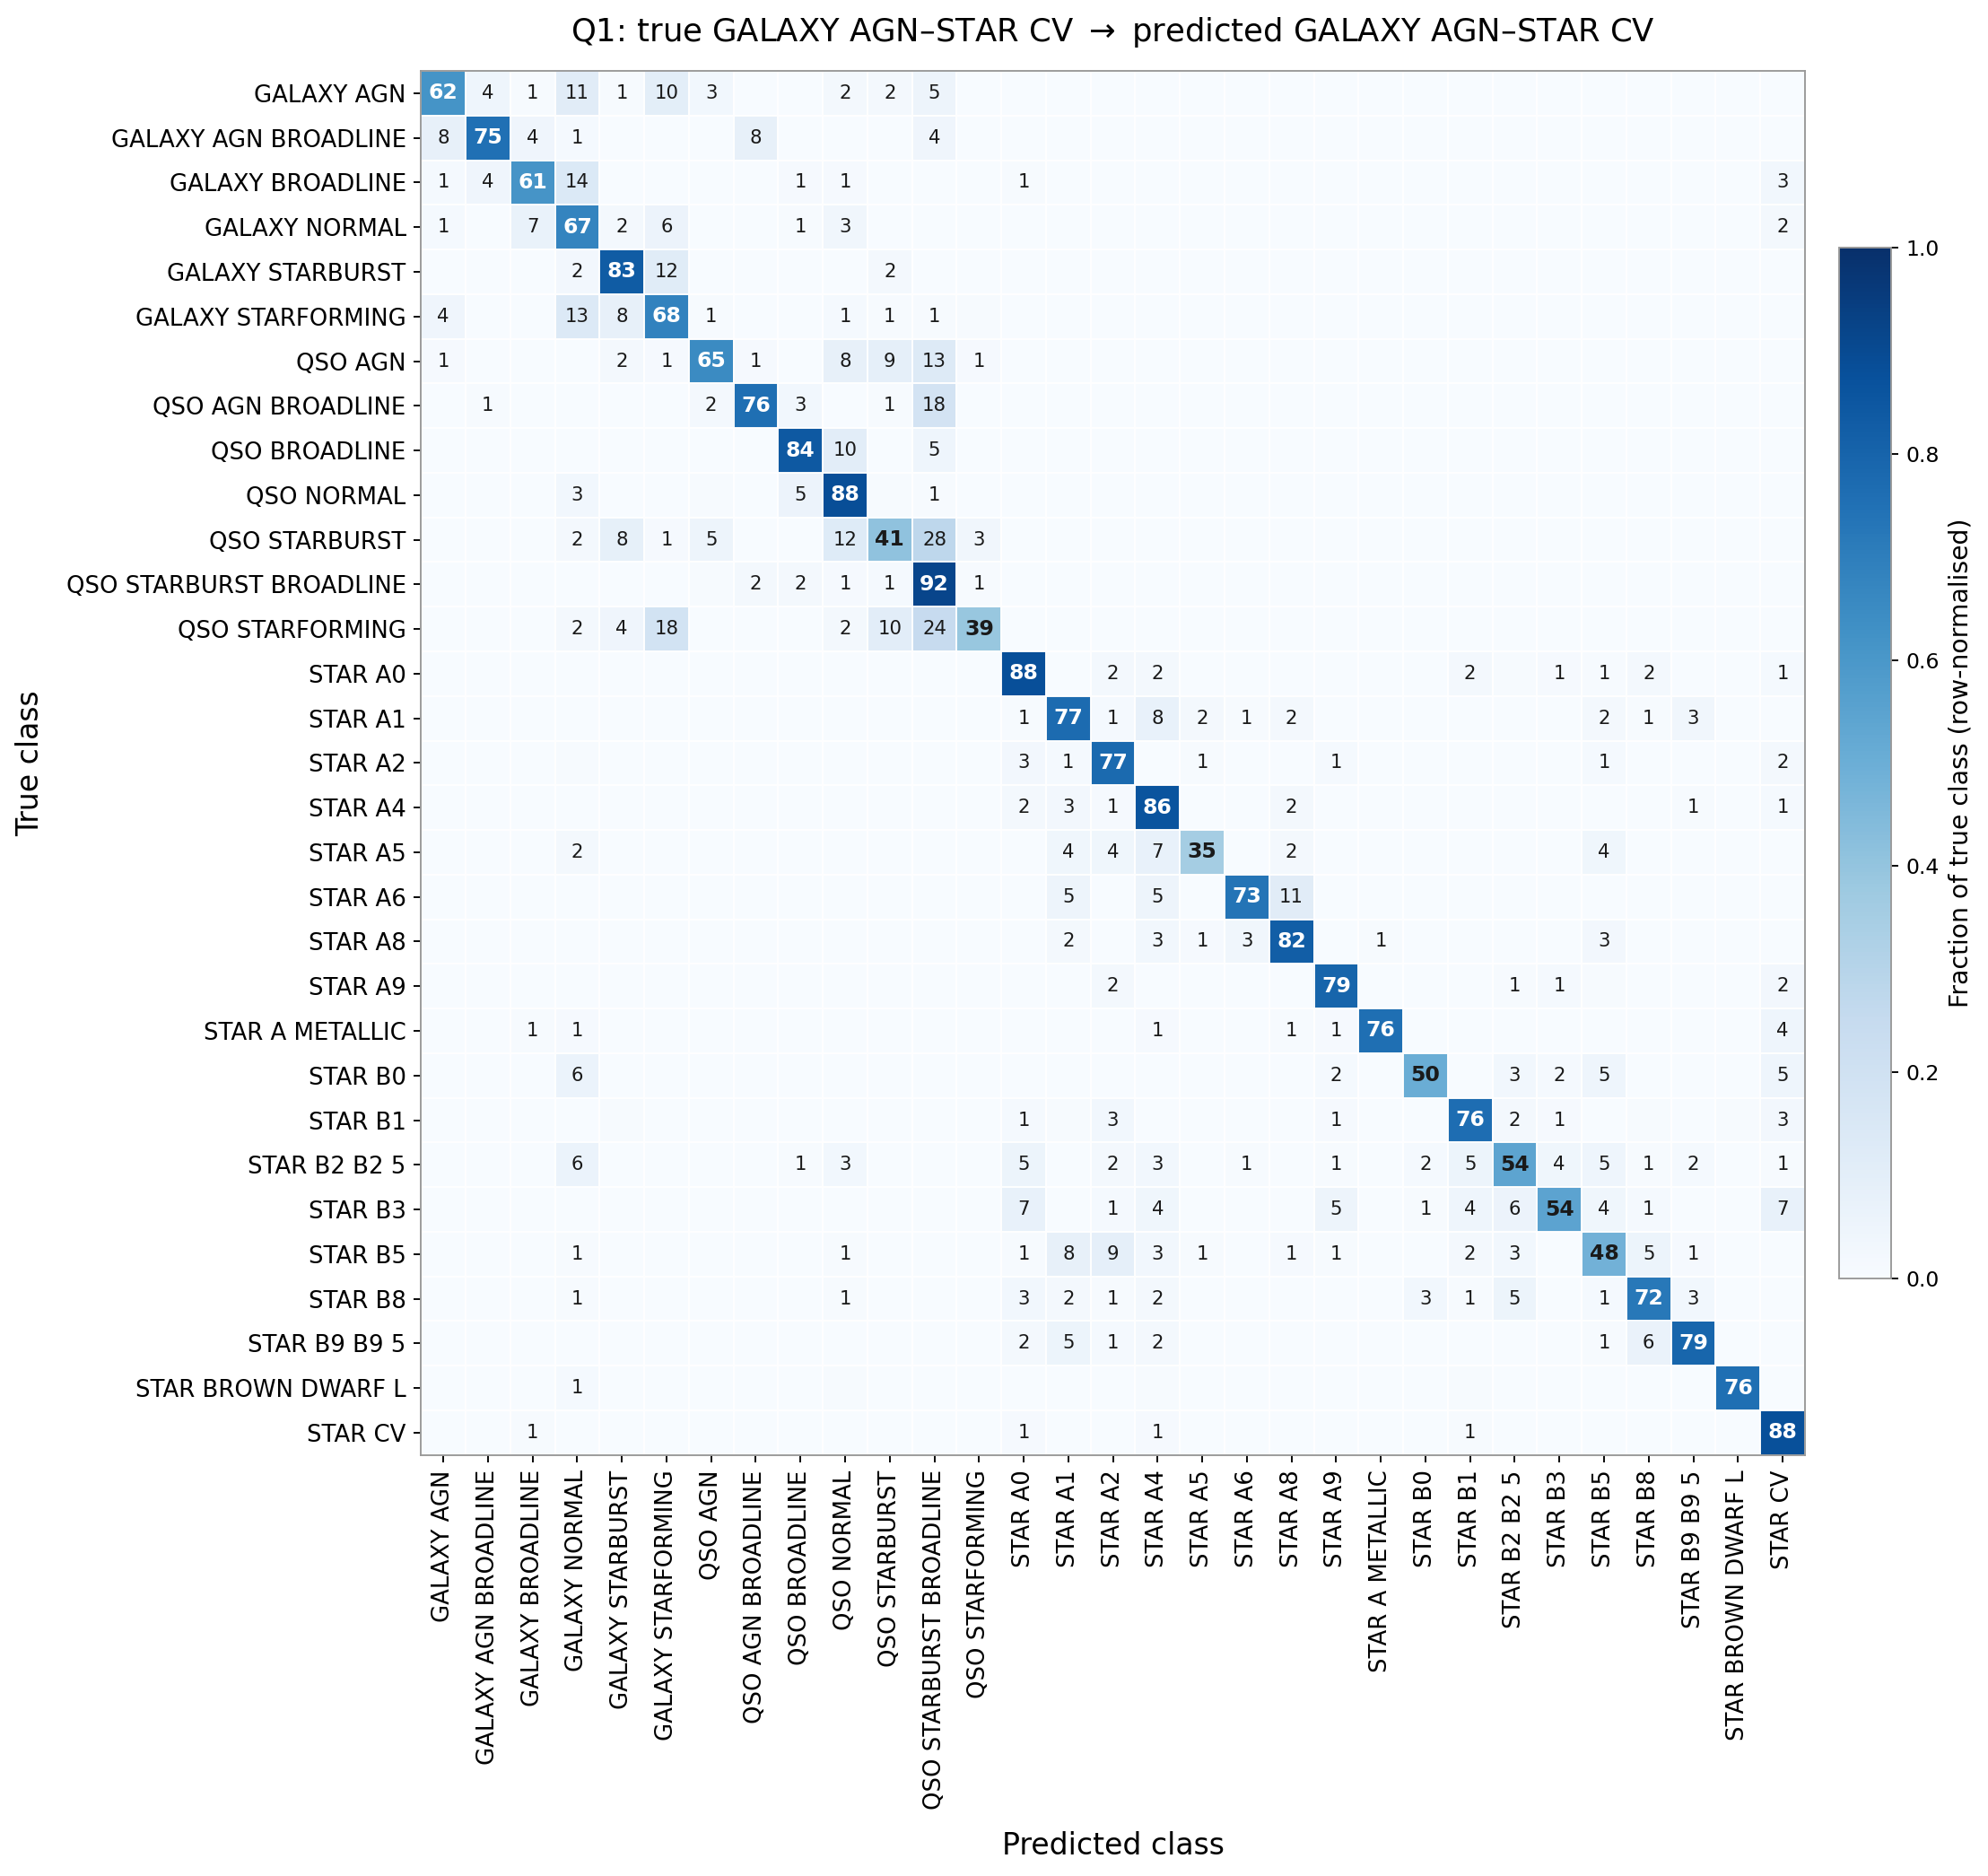
\includegraphics[width=0.96\textwidth]{Figures/cm_cnn_baseline_q1.png}
    \caption{Quadrant 1 of the 62-class Baseline CNN confusion matrix: true and
        predicted classes both from the first half of the class list
        (\texttt{GALAXY\_AGN} through \texttt{STAR\_CV}). This block contains the
        extragalactic classes and the hot and exotic stellar types. Values are
        percentages of each true class; cells below $0.5\%$ are left blank.}
    \label{fig:cm_baseline_q1}
\end{figure*}

\begin{figure*}[htbp]
    \centering
    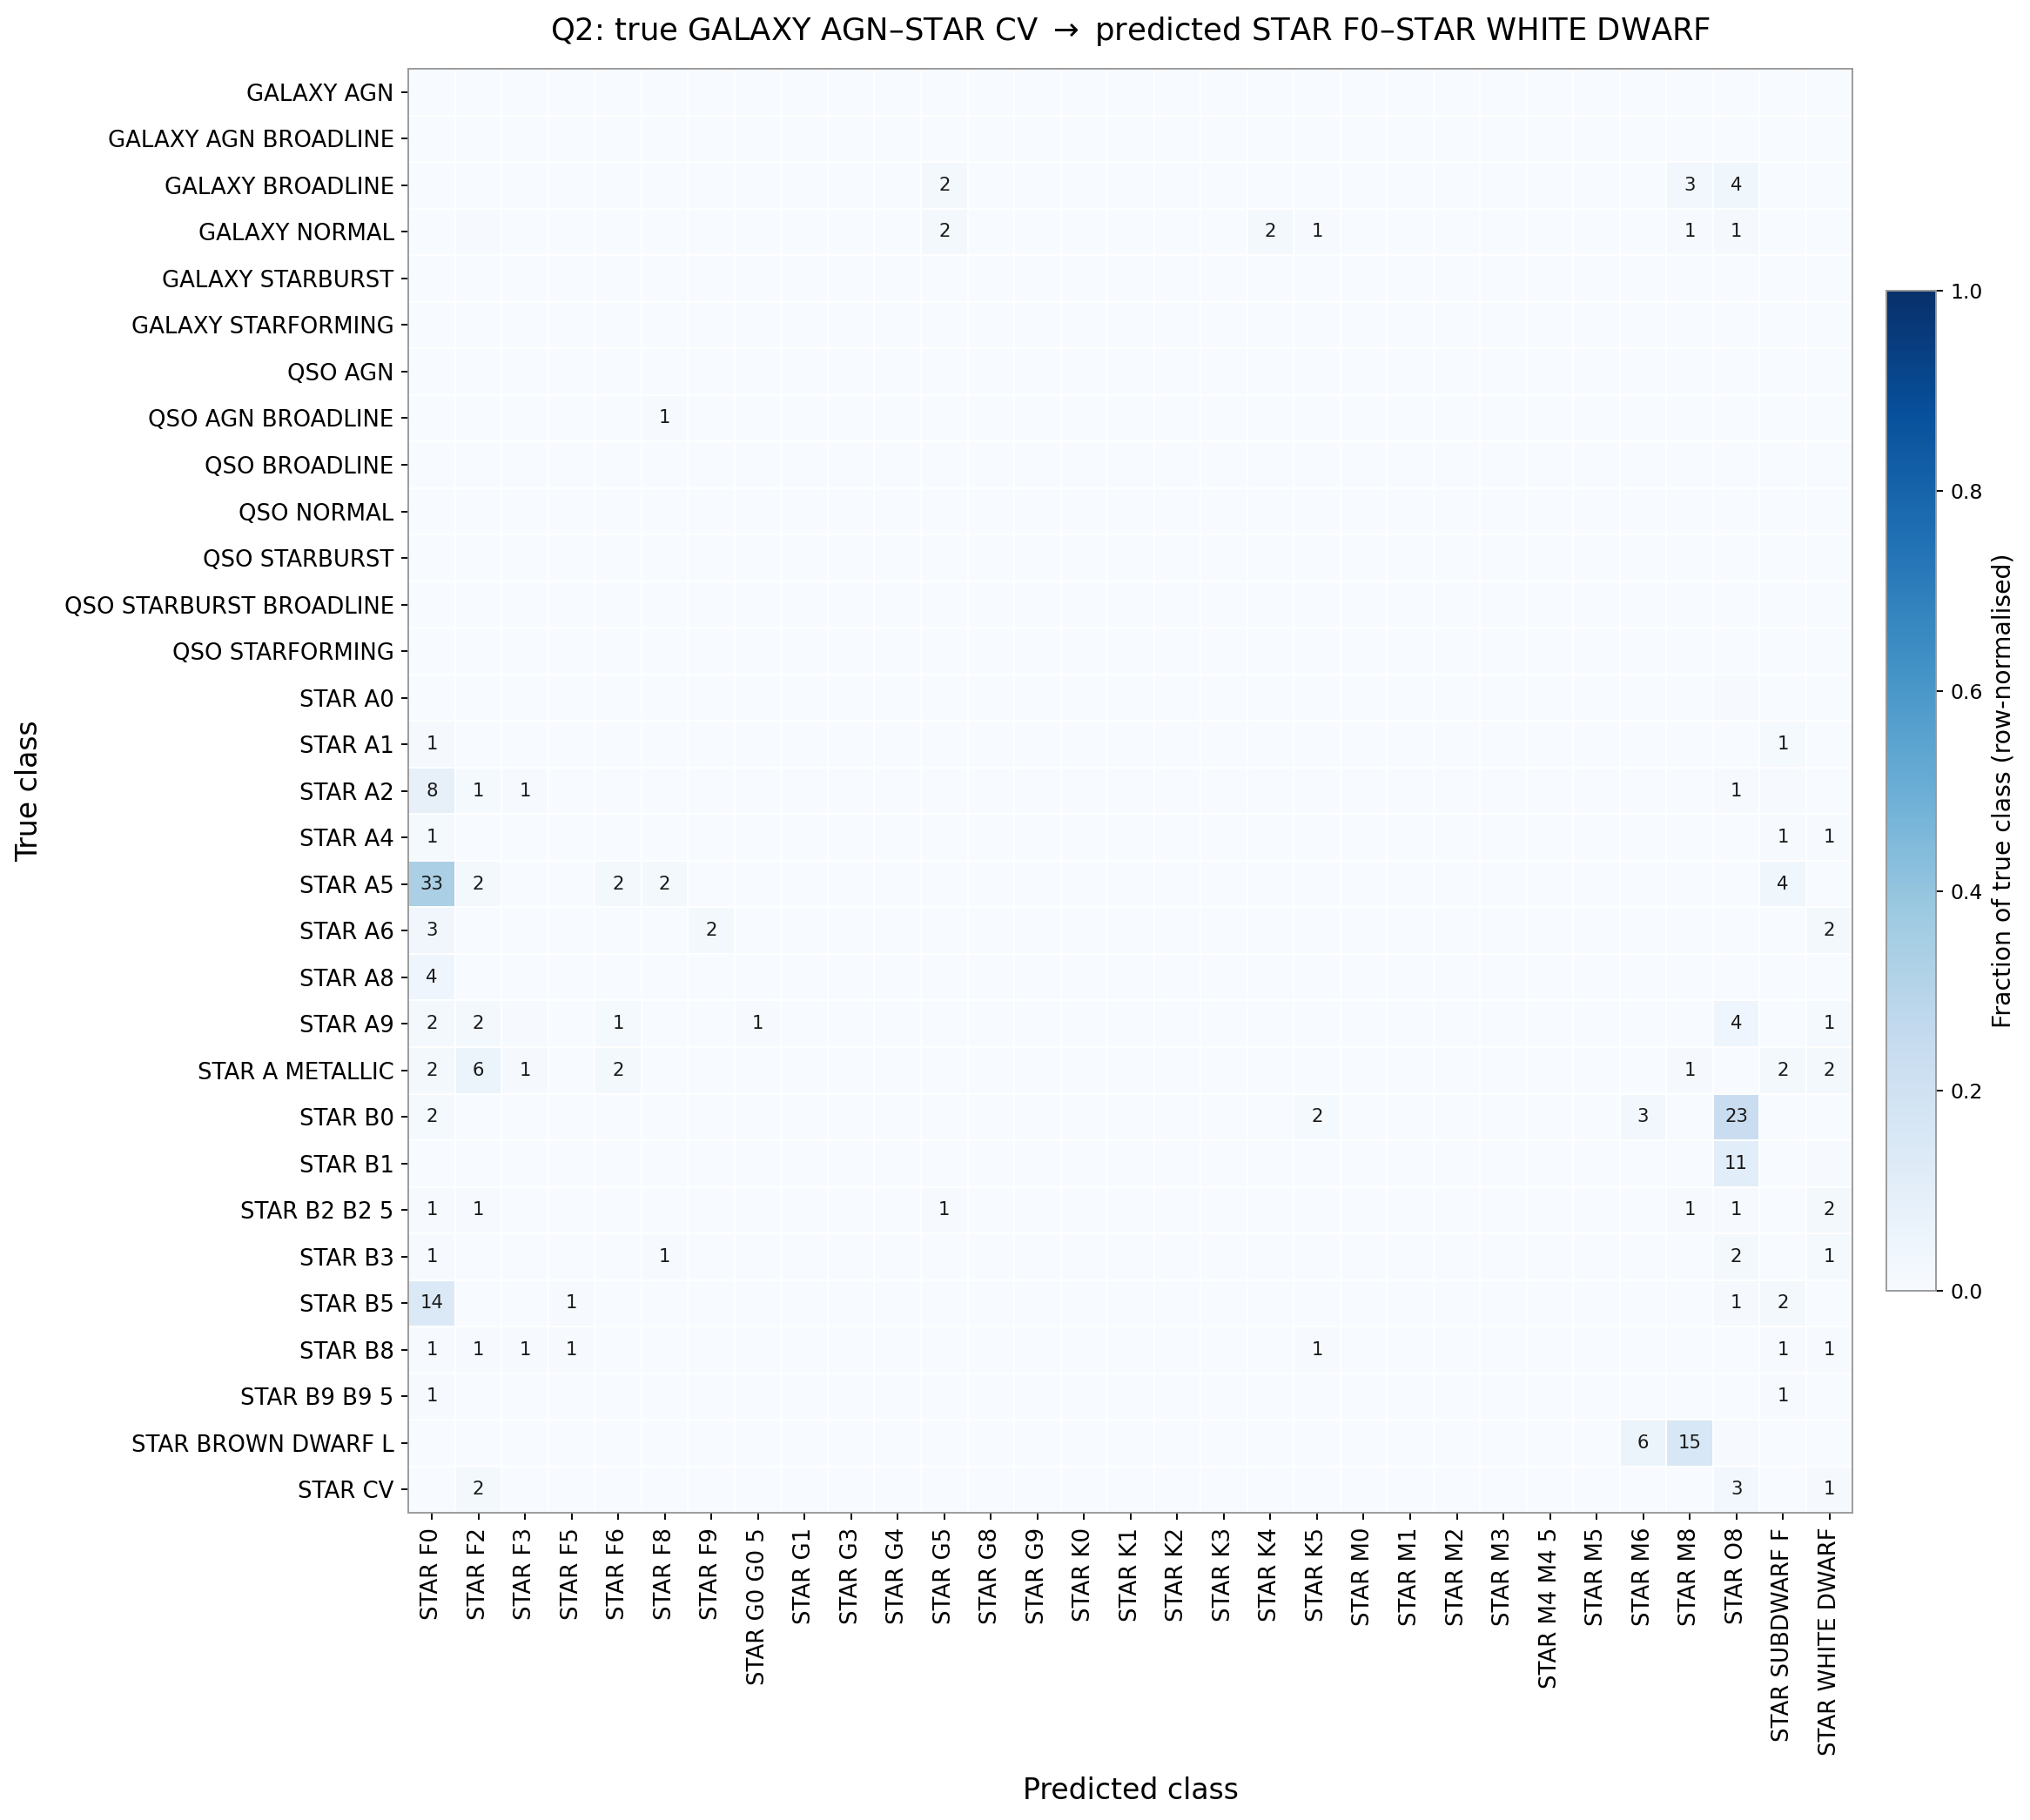
\includegraphics[width=0.96\textwidth]{Figures/cm_cnn_baseline_q2.png}
    \caption{Quadrant 2: true classes from the first half, predicted classes from
        the second half (\texttt{STAR\_F0} through \texttt{STAR\_WHITE\_DWARF}).
        The block is sparse, showing that the extragalactic classes are
        essentially never mistaken for cool stars, and what mass it does carry is
        confined to a few stellar rows whose true neighbours happen to fall in the
        other half of the alphabetical ordering: \texttt{STAR\_A5} $\rightarrow$
        \texttt{STAR\_F0} ($33.3\%$), \texttt{STAR\_B0} $\rightarrow$
        \texttt{STAR\_O8} ($22.7\%$), \texttt{STAR\_BROWN\_DWARF\_L} $\rightarrow$
        \texttt{STAR\_M8} ($15.4\%$) and \texttt{STAR\_B5} $\rightarrow$
        \texttt{STAR\_F0} ($13.8\%$). The third of these is the pair that defines
        the binary task of Experiment~1.}
    \label{fig:cm_baseline_q2}
\end{figure*}

\begin{figure*}[htbp]
    \centering
    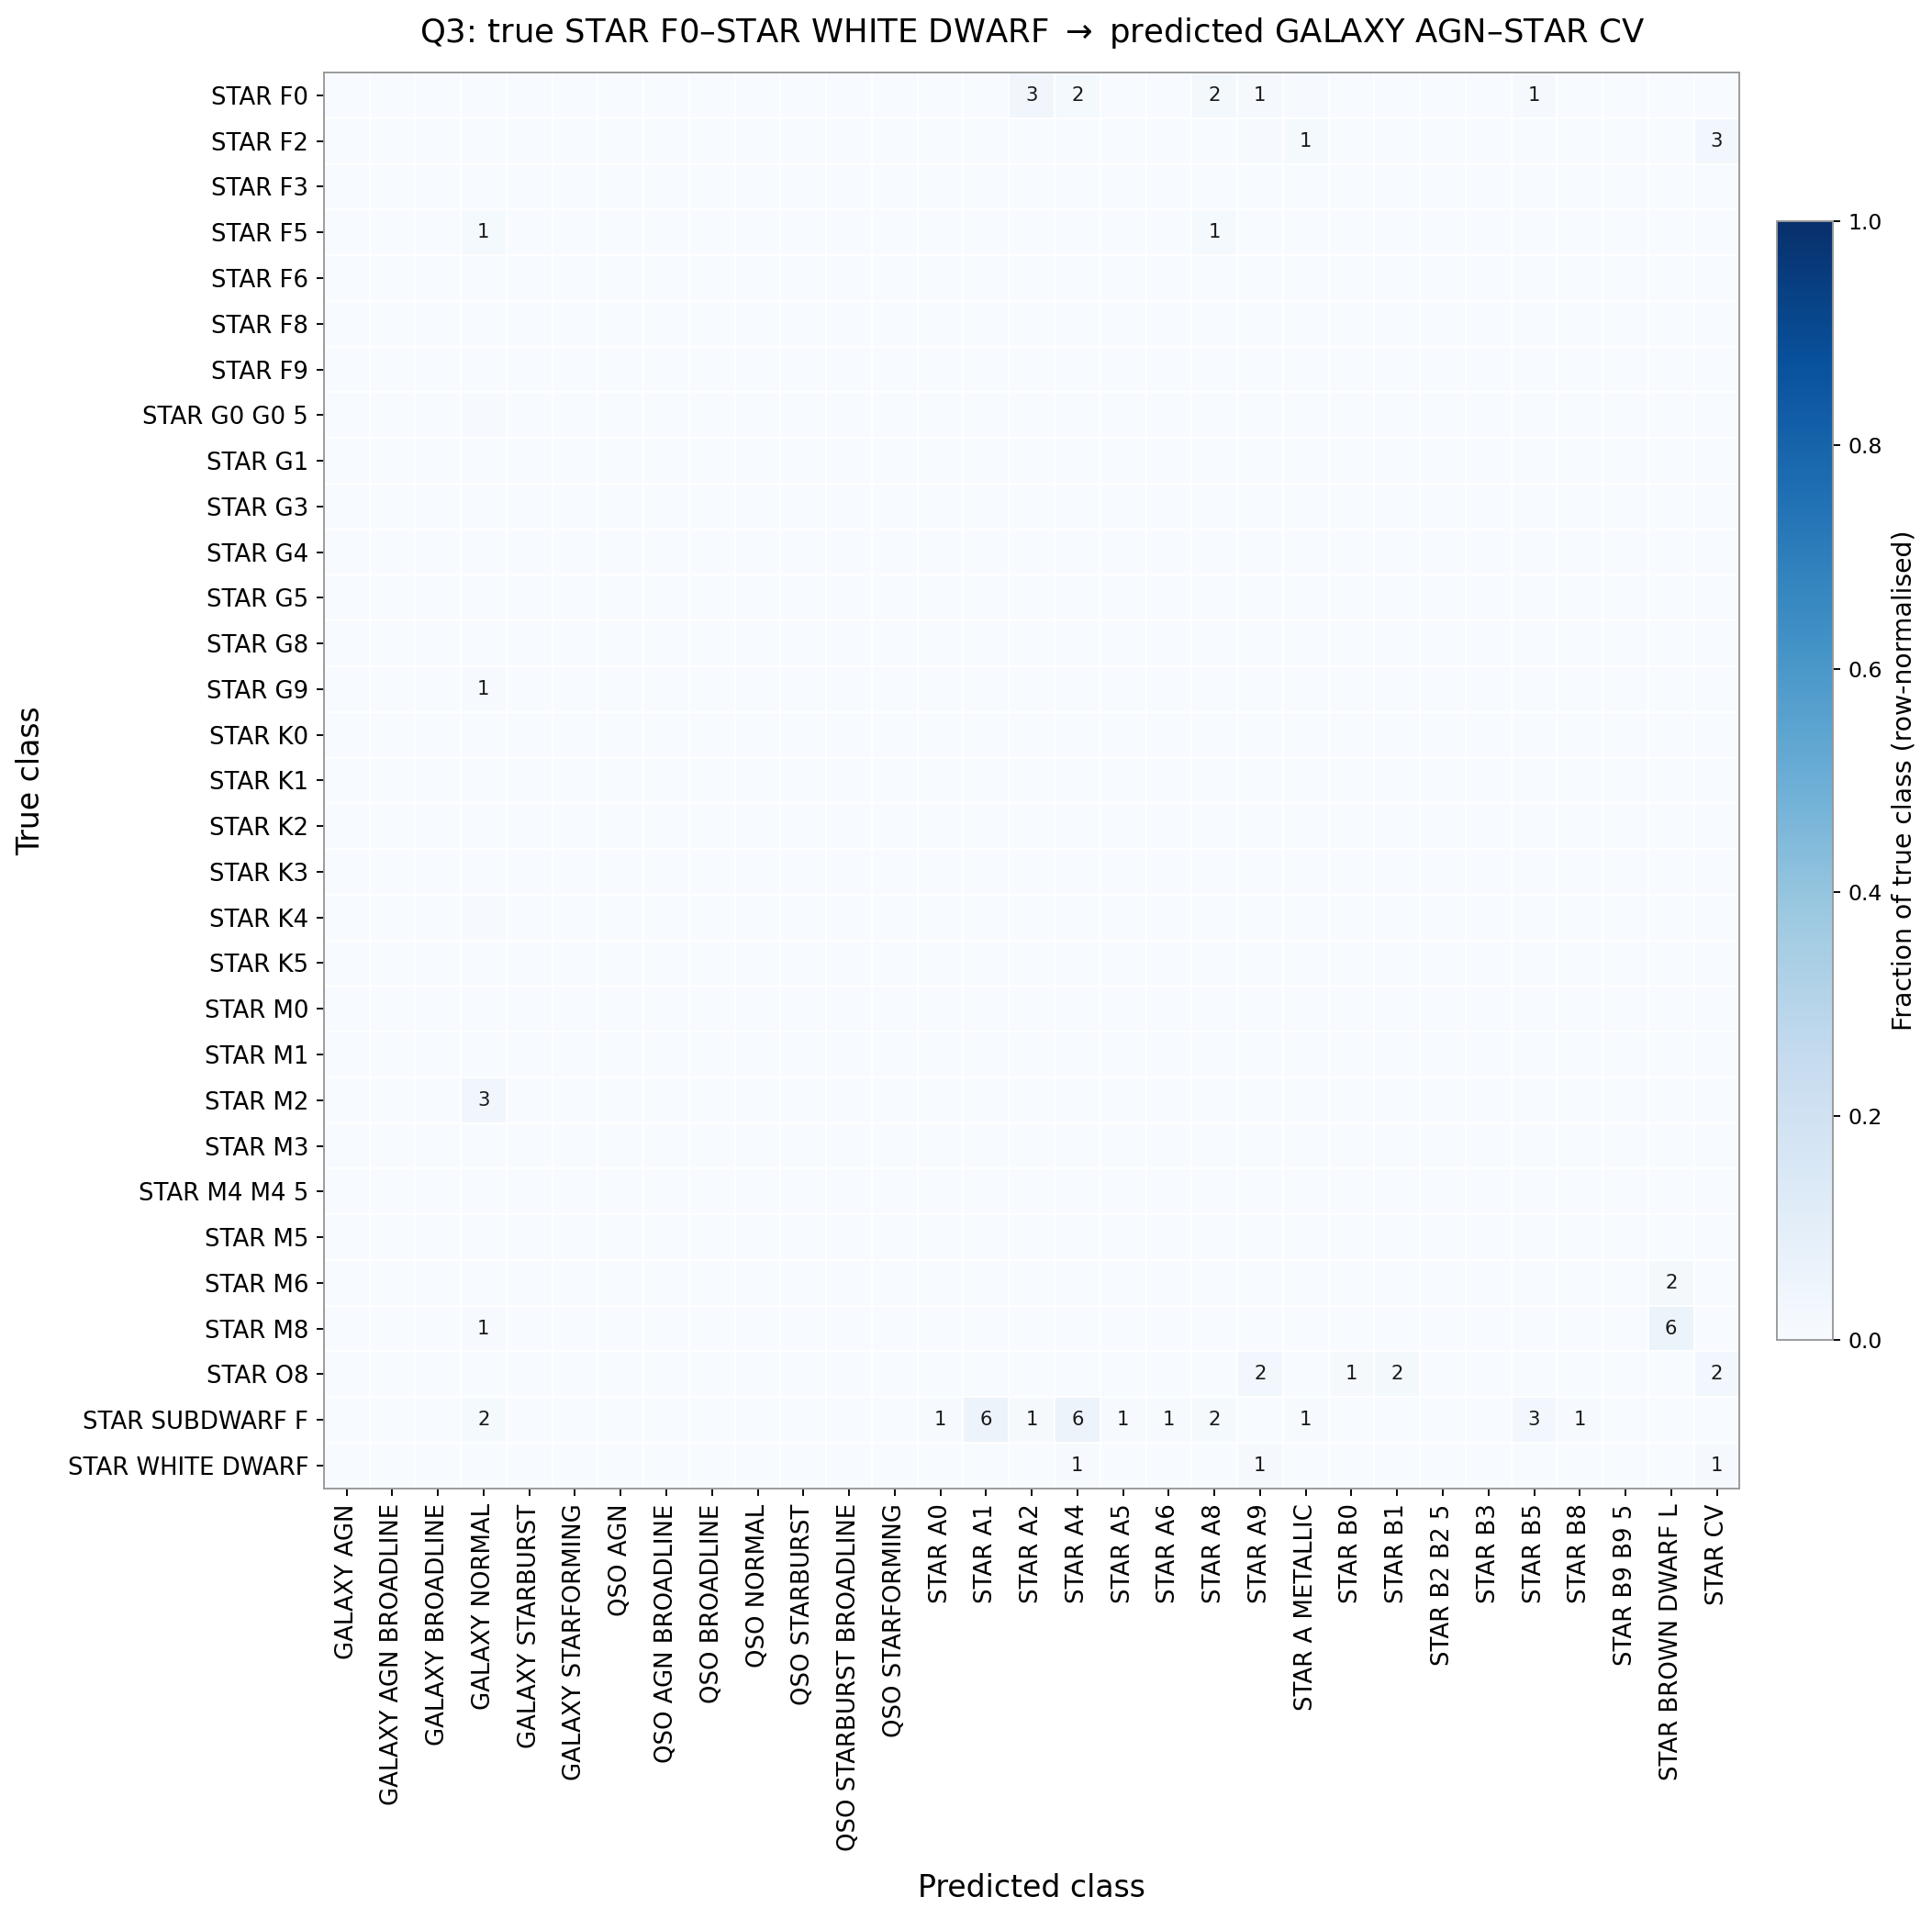
\includegraphics[width=0.96\textwidth]{Figures/cm_cnn_baseline_q3.png}
    \caption{Quadrant 3: true classes from the second half, predicted classes
        from the first half. This is the sparsest of the four blocks, carrying
        only $0.75$ of the total row mass of $62$, which confirms that cool
        stellar types are almost never assigned to extragalactic or hot-star
        labels.}
    \label{fig:cm_baseline_q3}
\end{figure*}

\begin{figure*}[htbp]
    \centering
    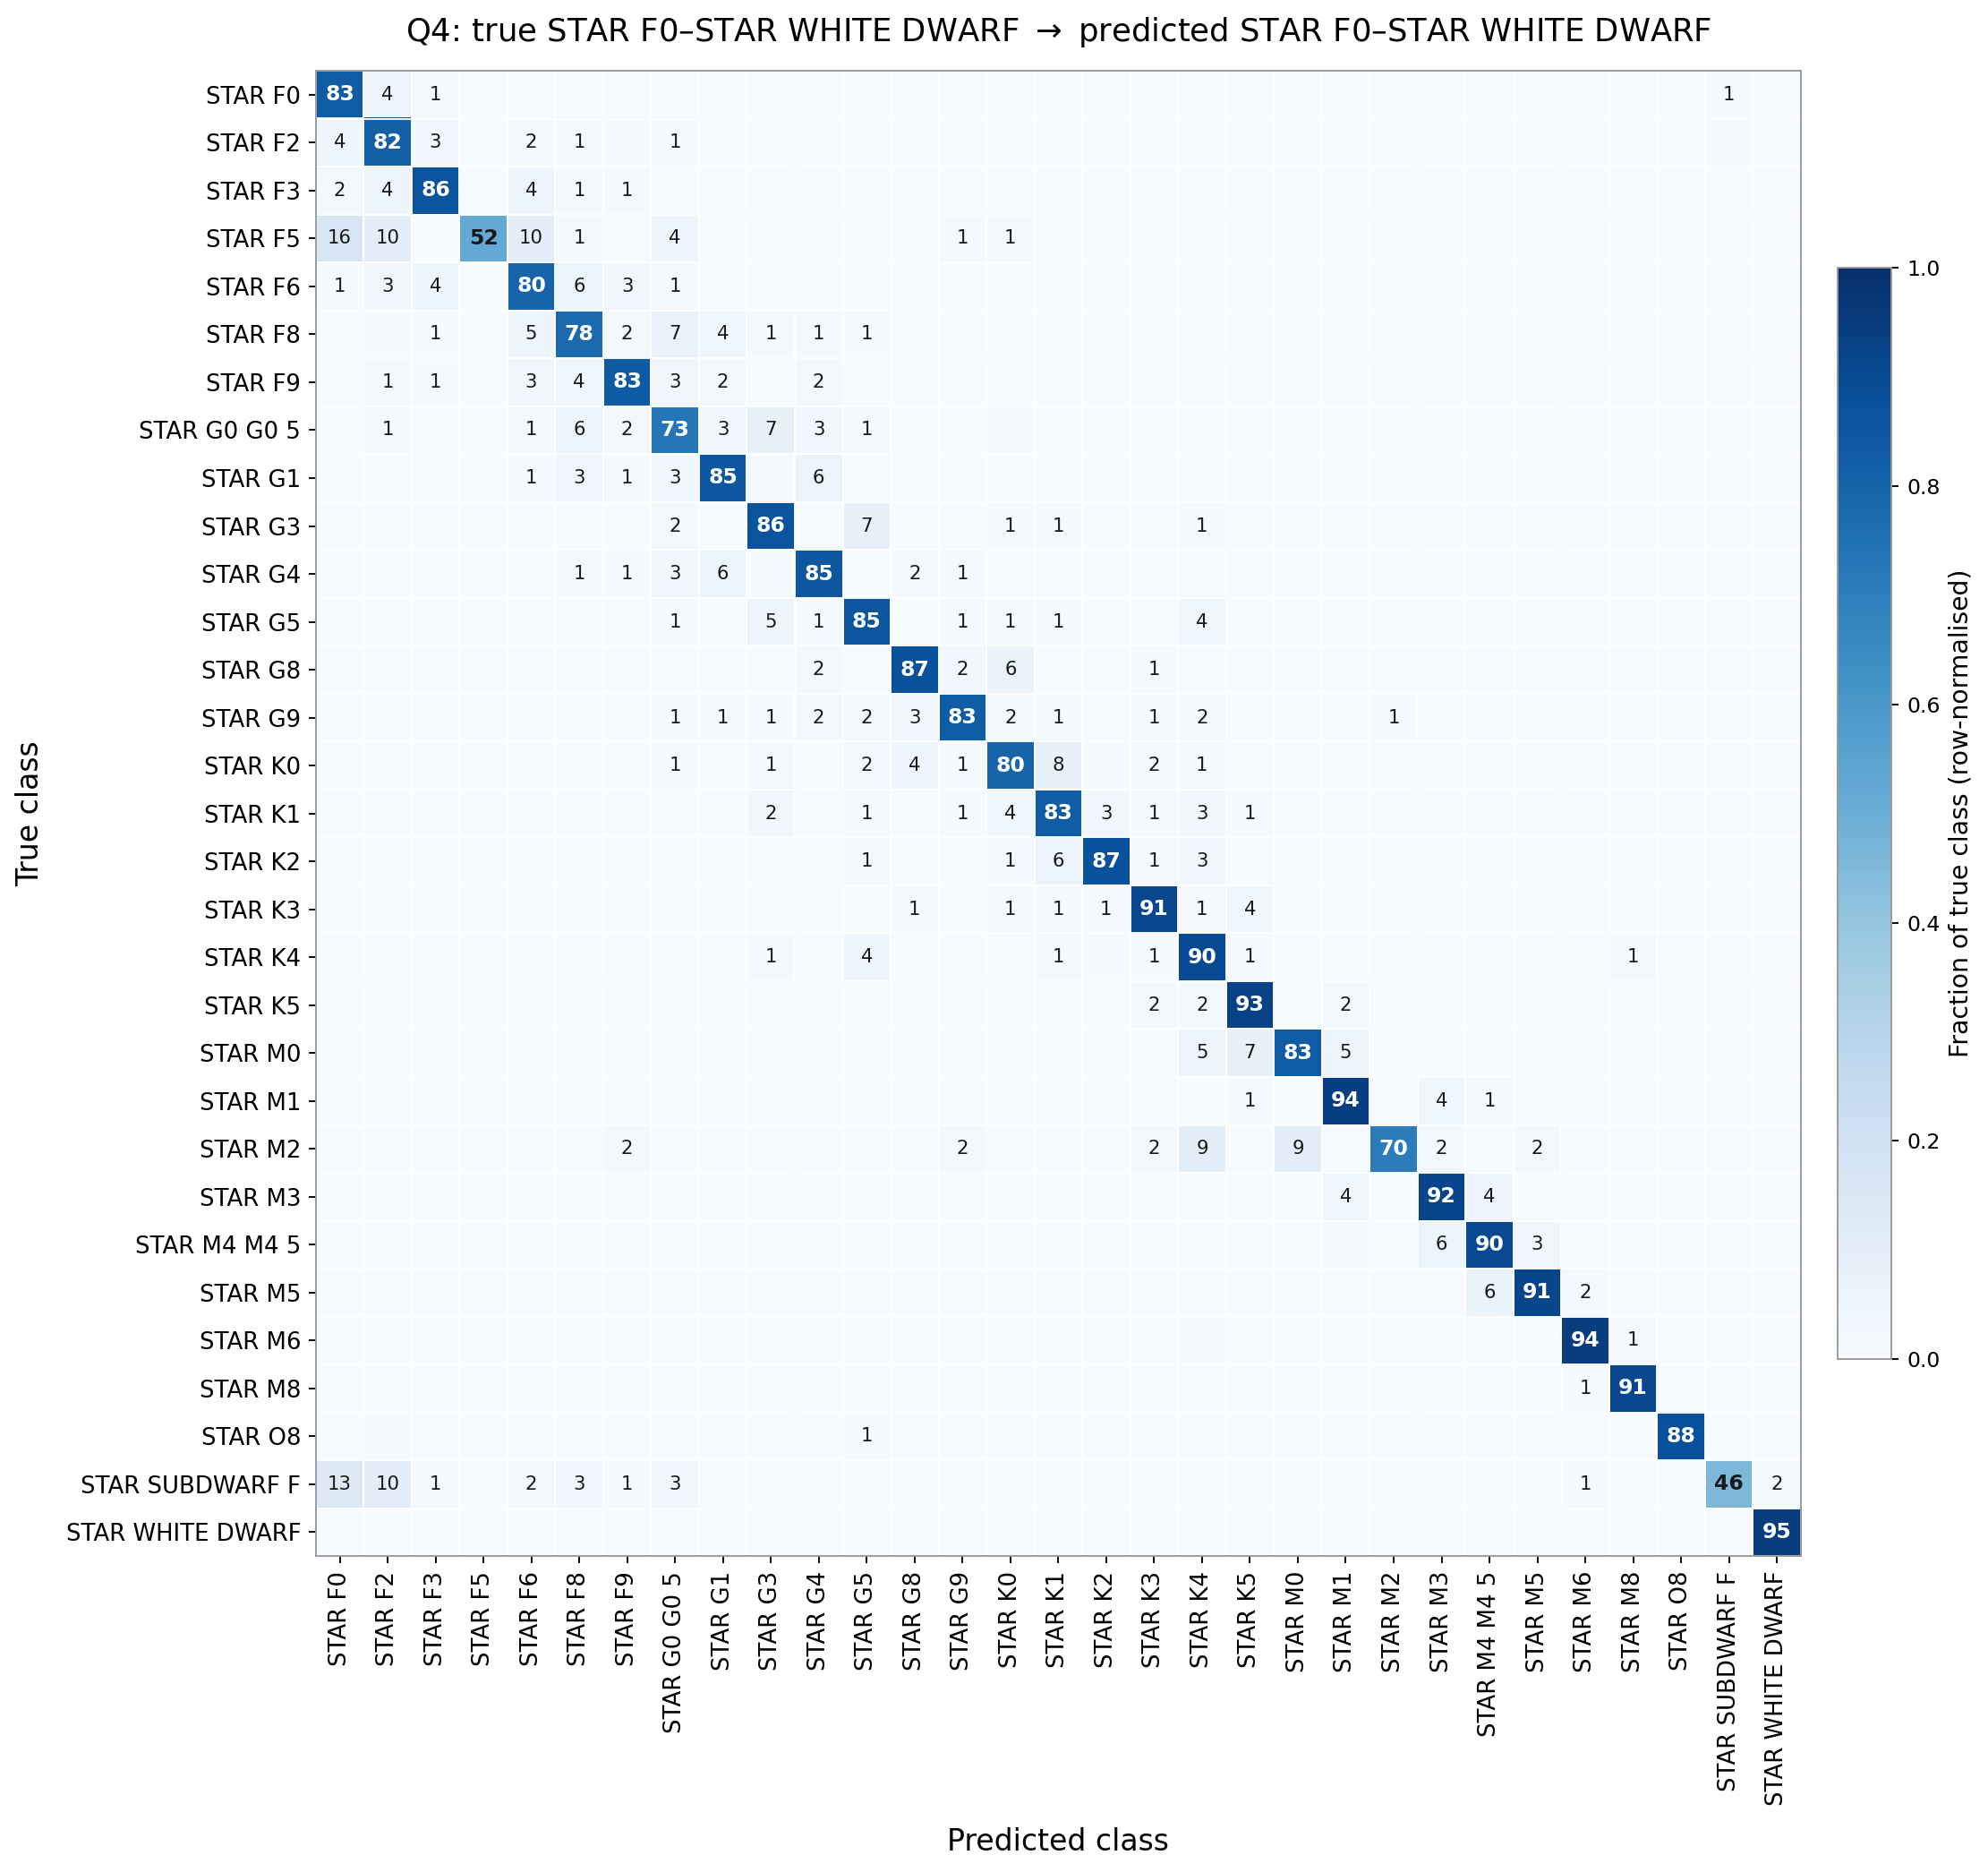
\includegraphics[width=0.96\textwidth]{Figures/cm_cnn_baseline_q4.png}
    \caption{Quadrant 4: true and predicted classes both from the second half of
        the class list (\texttt{STAR\_F0} through \texttt{STAR\_WHITE\_DWARF}).
        The confusion is concentrated tightly around the diagonal, reflecting the
        continuous temperature sequence of the F, G, K and M types, where each
        class is confused almost exclusively with its immediate neighbours.}
    \label{fig:cm_baseline_q4}
\end{figure*}
